\section{度量空间的比较}
\label{sec:metric-comparison}

上一节固定映射，研究它的连续性；本节反过来，用映射比较两个度量空间：如果两个空间之间有一个足够好的对应，一侧的柯西列、完备性和开集能否搬到另一侧？比较的强弱取决于对应保留了什么。等距与双Lipschitz映射双向控制距离的数值，同胚只要求双向连续。同一底集上的两个度量，也可以借恒等映射按这两种要求比较。

\subsection{等距与双Lipschitz映射}
\label{sec:metric-bilipschitz}

最强的比较是距离完全不变。把平面上的图形平移或旋转，所有两点距离都保持不变；把一个空间放进它的完备化，原有距离也不变。

\begin{definition}[等距与双Lipschitz映射]
\label{def:metric-bilipschitz}
设$f:D\to Y$，$D\subseteq X$。若存在常数$0<c\leq C<\infty$，使所有$x,y\in D$满足
\begin{equation}
\label{eq:metric-bilipschitz}
  c\,d_X(x,y)\leq d_Y(f(x),f(y))\leq C\,d_X(x,y),
\end{equation}
就称$f$为\term{双Lipschitz映射}（bi-Lipschitz map）。$c=C=1$，即$d_Y(f(x),f(y))=d_X(x,y)$时，称$f$为\term{等距映射}（isometry）。
\end{definition}

上界说明$f$是Lipschitz映射，控制正向误差。下界有两个作用：若$f(x)=f(y)$，则$c\,d_X(x,y)\leq0$，于是$x=y$，所以$f$是单射；并且逆映射$f^{-1}:f(D)\to D$满足$d_X(f^{-1}(u),f^{-1}(v))\leq c^{-1}d_Y(u,v)$，是常数为$1/c$的Lipschitz映射。逆映射只在实际像$f(D)$上有定义；只有当$f$还是满射时，才能说它在整个$Y$上可逆。

\begin{example}[有限维范数之间的恒等映射]
\label{ex:metric-identity-bilipschitz}
在$\mathbb R^d$上，对每个$\bm x$有$\lVert\bm x\rVert_2\leq\lVert\bm x\rVert_1\leq\sqrt d\,\lVert\bm x\rVert_2$，其中右边一式来自Cauchy--Schwarz不等式$\sum_i|x_i|\cdot1\leq\bigl(\sum_ix_i^2\bigr)^{1/2}\sqrt d$。所以恒等映射$(\mathbb R^d,d_2)\to(\mathbb R^d,d_1)$是双Lipschitz映射，$c=1$，$C=\sqrt d$。$d=2$时，取$\bm x=(1,1)$，$\lVert\bm x\rVert_1=2=\sqrt2\,\lVert\bm x\rVert_2$，上界取等号，这个常数不能再小。
\end{example}

\paragraph{双Lipschitz映射保留的性质}
由式~\eqref{eq:metric-bilipschitz}，$d_X(x_m,x_n)$与$d_Y(f(x_m),f(x_n))$同时趋于零，所以$(x_n)$是$D$中的柯西列当且仅当$(f(x_n))$是$f(D)$中的柯西列，$x_n\to x$当且仅当$f(x_n)\to f(x)$。由此，$D$完备当且仅当$f(D)$完备：若$D$完备，$f(D)$中的柯西列$(f(x_n))$对应$D$中的柯西列$(x_n)$，它收敛到某个$x\in D$，于是$f(x_n)\to f(x)\in f(D)$；反方向对逆映射作同样论证。全有界性也相互对应：$\{a_1,\dots,a_k\}$是$D$的$\varepsilon$网时，$\{f(a_1),\dots,f(a_k)\}$是$f(D)$的$C\varepsilon$网；反过来，$f(D)$的$\varepsilon$网对应$D$的$\varepsilon/c$网。这些比较都针对实际像$f(D)$；若$f$不是满射，陪域$Y$中$f(D)$以外的部分不受约束。

图~\ref{fig:metric-bilipschitz-homeo}(a)用例~\ref{ex:metric-identity-bilipschitz}中的常数画出了双Lipschitz映射的特点：输出距离被夹在两条过原点的直线之间。

\subsection{同胚与度量的比较}
\label{sec:metric-homeomorphism}

很多问题只关心收敛与开集，不关心误差的比例。例如判断一个点列是否收敛、一个集合是否开，只需知道哪些点“任意接近”，不必知道接近的速度。

\begin{definition}[同胚]
\label{def:metric-homeomorphism}
若双射$h:X\to Y$与它的逆映射$h^{-1}:Y\to X$都连续，就称$h$为\term{同胚}（homeomorphism），称$X$与$Y$同胚。
\end{definition}

由开集原像判据，同胚把$X$的开集恰好对应到$Y$的开集：$U$在$X$中开时，$h(U)=(h^{-1})^{-1}(U)$在$Y$中开，反之亦然。由序列判据，$x_n\to x$当且仅当$h(x_n)\to h(x)$。所以同胚保留开集、闭集、闭包、收敛与连续性这些只依赖开集的结构。双Lipschitz双射的两个方向都是Lipschitz映射，因而都连续，必为同胚；反之则不然，下面的例子说明同胚不必保持距离的比例。

\paragraph{同一底集上的两种度量}
若$d$与$d'$是同一集合$X$上的两个度量，恒等映射$(X,d)\to(X,d')$是同胚，当且仅当两个度量给出相同的开集；这时称两个度量\term{拓扑等价}（topologically equivalent）。若恒等映射还是双Lipschitz的，即存在$0<c\leq C$使$c\,d\leq d'\leq C\,d$，就称它们\term{强等价}（strongly equivalent）。例~\ref{ex:metric-identity-bilipschitz}说明$d_1$与$d_2$强等价；第~\ref{sec:metric-definition}节的$\rho_1$与$\rho_\infty$由式~\eqref{eq:metric-product-bounds}也强等价。而$\mathbb R$上的通常距离与离散度量不拓扑等价：$\{0\}$在离散度量下开，在通常距离下不开。这里只讨论度量诱导的开集，不展开一般拓扑空间的公理体系。

\begin{example}[logit同胚与完备性]
\label{ex:metric-logit}
令$h:(0,1)\to\mathbb R$，$h(x)=\ln\dfrac{x}{1-x}$，两端都取通常距离。它是严格单调的连续双射，逆映射是$\sigma(t)=1/(1+\mathrm e^{-t})$，也连续，所以$h$是同胚。$(0,1)$不完备，$\mathbb R$完备；同胚没有保留完备性。原因在于$h$不是双Lipschitz映射：柯西列$x_n=1/(n+1)$的像$h(x_n)=\ln\dfrac{1/(n+1)}{n/(n+1)}=-\ln n$满足$|h(x_{2n})-h(x_n)|=\ln2$，对任何$N$都有相距$\ln2$的两项，所以$(h(x_n))$不是柯西列。具体地，$h(x_1),\dots,h(x_4)$依次为$0,\ -0.693,\ -1.099,\ -1.386$，而$x_1,\dots,x_4$之间的距离越来越小。图~\ref{fig:metric-bilipschitz-homeo}(b)画出了这种拉伸：同胚保留“哪些点列收敛”，却可以把一列趋向缺失端点的柯西列拉成无界的点列。
\end{example}

\begin{figure*}[!htbp]
  \centering
  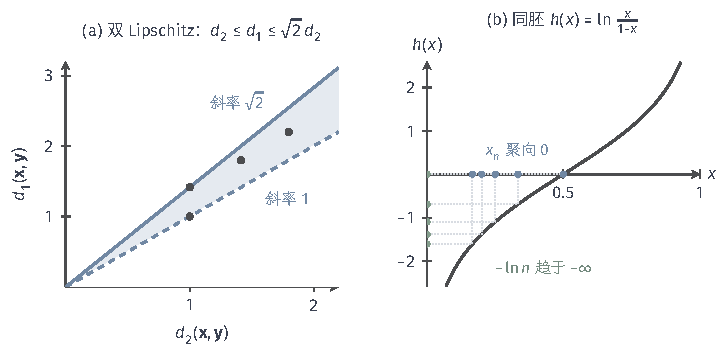
\includegraphics[width=123.261mm]{figures/02-abstract-mathematics/01-metric-and-measure/tikz/c1-bilipschitz-homeo/figure.pdf}
  \caption{双Lipschitz映射与同胚的区别。(a) 恒等映射$(\mathbb R^2,d_2)\to(\mathbb R^2,d_1)$：横轴为输入距离$d_2$，纵轴为输出距离$d_1$，所有点对都落在斜率$1$与$\sqrt2$两条直线之间的蓝色楔形中，输出误差与输入误差相差不超过常数倍。(b) logit同胚$h(x)=\ln(x/(1-x))$：横轴上的蓝点$x_n=1/(n+1)$（$n=1,\dots,5$）向$0$聚拢，构成柯西列，纵轴上的像$-\ln n$却越拉越远并趋于$-\infty$。}
  \label{fig:metric-bilipschitz-homeo}
\end{figure*}

这个例子同时说明，完备性不是只由开集决定的性质：$\mathbb R$上的通常距离$|s-t|$与$d'(s,t)=|\sigma(s)-\sigma(t)|$给出相同的开集（$\sigma:\mathbb R\to(0,1)$是同胚），但$(\mathbb R,|\cdot|)$完备，而在$d'$下点列$t_n=n$满足$d'(t_m,t_n)=|\sigma(m)-\sigma(n)|\to0$，是柯西列，却没有极限：若在$d'$下$t_n\to t$，则$\sigma(n)\to\sigma(t)<1$，与$\sigma(n)\to1$矛盾。讨论完备性、全有界性以及下一节的压缩条件时，必须指明所用的度量；只说“拓扑相同”不够。
